\documentclass{article}

\usepackage{graphicx}
\usepackage{tikz}
\usepackage{tikzsymbols}
\usetikzlibrary{calc,patterns,shapes.geometric}
\pagestyle{empty}
\usepackage[margin=0pt]{geometry}
\geometry{papersize={14in,12in}}

\def\centerarc[#1](#2)(#3:#4:#5){\draw[#1] ($(#2)+({#5*cos(#3)},{#5*sin(#3)})$) arc (#3:#4:#5);}

\begin{document}
	\begin{figure}
		\centering
		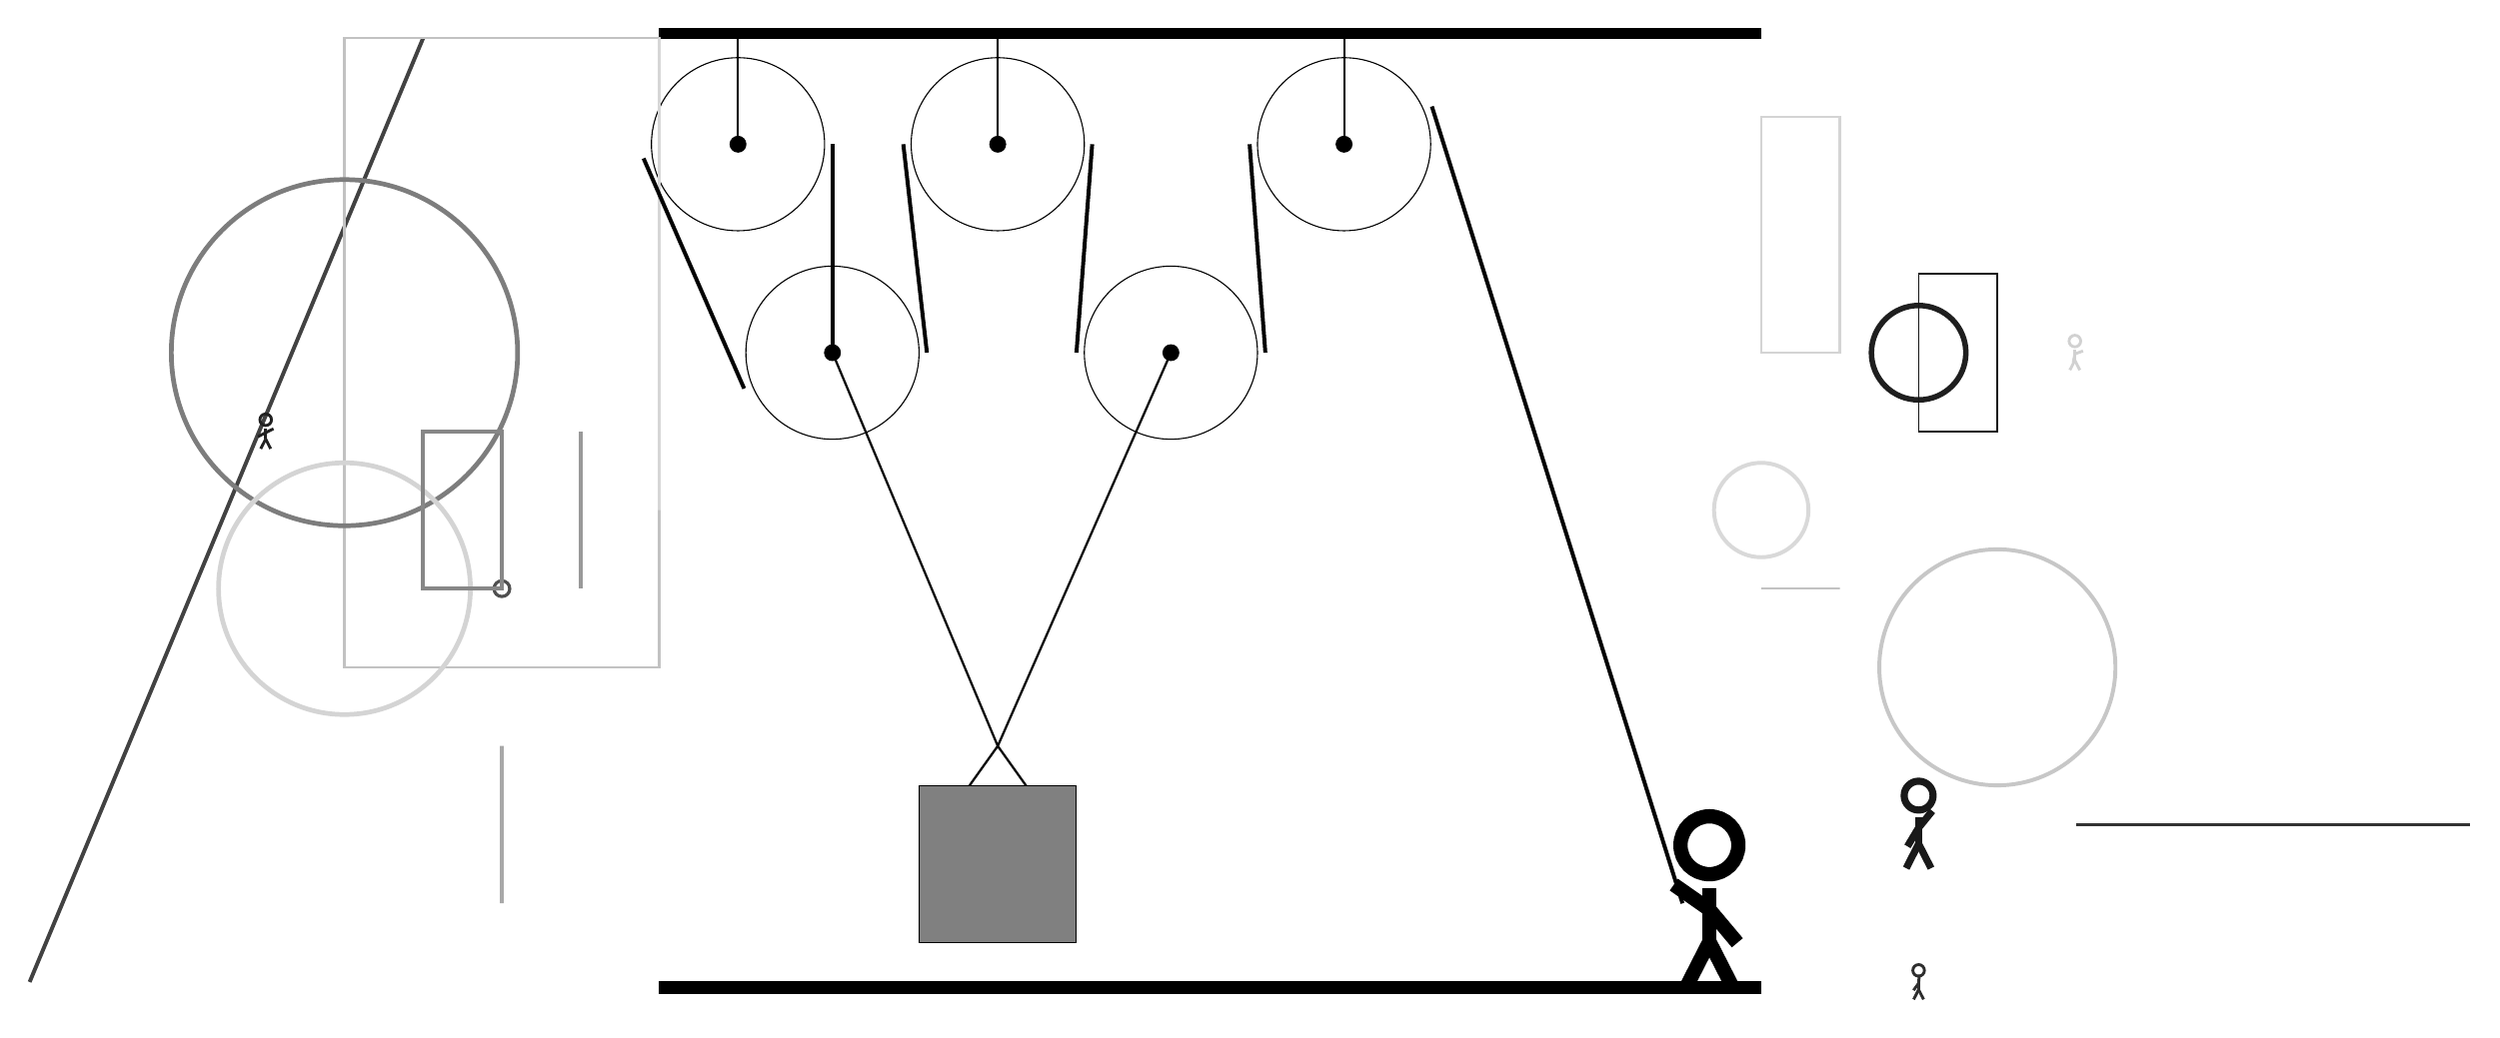
\begin{tikzpicture}
			%%%%% START %%%%%
			
			\draw[fill=black] (-2, 9) rectangle (12, 9.125);
			
			\draw (-1, 7.65) circle (1.1);
			\draw[fill=black] (-1, 7.65) circle (0.1);
			\draw[thick] (-1, 7.65) -- (-1, 9);
			
			\draw (2.3, 7.65) circle (1.1);
			\draw[fill=black] (2.3, 7.65) circle (0.1);
			\draw[thick] (2.3, 7.65) -- (2.3, 9);
			
			\draw (6.7, 7.65) circle (1.1);
			\draw[fill=black] (6.7, 7.65) circle (0.1);
			\draw[thick] (6.7, 7.65) -- (6.7, 9);
			
			\draw (0.2, 5) circle (1.1);
			\draw[fill=black] (0.2, 5) circle (0.1);
			
			\draw[line width=0.5mm, color=black!74](-5, 9) -- (-10, -3);
			
			\draw[line width=0.5mm, color=black!34] (-4, 0) rectangle (-4, -2);
			\draw[line width=0.3mm, color=black!24] (-2, 9) rectangle (-6, 1);
			\draw[line width=0.3mm, color=black!24] (13, 2) rectangle (12, 2);
			\draw[line width=0.3mm, color=black!17] (12, 8) rectangle (13, 5);
			\draw [line width=0.5mm, color=black!15](12, 3) circle (0.6);
			
			\draw [line width=0.7mm, color=black!88](14, 5) circle (0.6);
			
			\node[line width=0.5mm, color=black!18] at (16, 5) {\Strichmaxerl[2][79][20]};
			\draw [line width=0.5mm, color=black!22](15, 1) circle (1.5);
			\draw [line width=0.6mm, color=black!51](-6, 5) circle (2.2);
			
			\node[line width=0.7mm, color=black!87] at (-7, 4) {\Strichmaxerl[2][28][26]};
			\draw[line width=0.2mm, color=black!91] (14, 4) rectangle (15, 6);
			\draw[line width=0.5mm, color=black!80](16, -1) -- (21, -1);
			\node[line width=0.2mm, color=black!90] at (14, -1) {\Strichmaxerl[5][59][51]};
			\draw [line width=0.4mm, color=black!69](-4, 2) circle (0.1);
			\draw[line width=0.3mm, color=black!16] (-2, 9) rectangle (-2, 3);
			
			\draw [line width=0.6mm, color=black!17](-6, 2) circle (1.6);
			\draw[line width=0.5mm, color=black!40](-3, 4) -- (-3, 2);
			\node[line width=0.7mm, color=black!82] at (14, -3) {\Strichmaxerl[2][54][85]};
			\draw[line width=0.5mm, color=black!47] (-4, 2) rectangle (-5, 4);
			
			\draw (4.5, 5) circle (1.1);
			\draw[fill=black] (4.5, 5) circle (0.1);
			
			\draw[thick] (0.2, 5) -- (2.3, 0)  -- (4.5, 5);
			\draw[thick]  (1.8, -0.7) -- (2.3, 0) -- (2.8, -0.7);
			\draw[fill=black!50] (1.3, -0.5) rectangle (3.3, -2.5);
			
			\draw[line width=0.5mm] (0.2, 5) -- (0.2, 7.65);
			\centerarc[line width=0.5mm](-1, 7.65)(0:200:1.2000000000000002);
			\draw[line width=0.5mm] (-2.2, 7.47) -- (-0.922, 4.544);
			\centerarc[line width=0.5mm](0.2, 5)(200:360:1.2000000000000002);
			\draw[line width=0.5mm](1.4, 5) -- (1.1, 7.65);
			\centerarc[line width=0.5mm](2.3, 7.65)(0:180:1.2000000000000002);
			\draw[line width=0.5mm] (3.5, 7.65) -- (3.3, 5);
			\centerarc[line width=0.5mm](4.5, 5)(180:360:1.2000000000000002);
			\draw[line width=0.5mm] (5.7, 5) -- (5.5, 7.65);
			\centerarc[line width=0.5mm](6.7, 7.65)(20:180:1.2000000000000002);
			\draw[line width=0.5mm](7.816, 8.13)  -- (11, -2);
			
			\node at (11.3, -2) {\Strichmaxerl[10][-35][-50]};
			
			\draw[fill=black] (-2, -3) rectangle (12, -3.15);
			
			%%%%% END %%%%%
		\end{tikzpicture}
	\end{figure}	
\end{document}